%!TEX root = ../thesis.tex
% appendix section 6

\chapter{Recombination continuum}
\label{sec:ap6}

Low-pressure dilute plasmas also exhibits continuum radiation. As the plasma is transparent (low opacity), the continuum radiation is not in the form of the blackbody spectrum. Here I introduce the recombination continuum that predominates the emission of laser plasma in low pressure gas ($\le 10 \text{ bar}$).

Reaction equation:
\begin{equation}
M^{+}+e\rightarrow M^{*}+h\nu
\end{equation}
The photon energy emitted from the recombination process is 
\begin{eqnarray}
h\nu & \equiv & E=\left|E_{n}\right|+\frac{1}{2}m_{e}v^{2}
\label{eq:photonEnergy}
\end{eqnarray}
, where $E_{n}$ is the energy difference between "ionization threshold" and $n$-th atomic level, $m_{e}$ is the electron mass and $v$ is the electron velocity. The radiation energy $dJ_{n}$ for a unit volume in a unit time from the recombination process that the ground state of the singly ionized ion $M^{+}$ captures the electron within the velocity interval from $v$ to $v+dv$ and becomes the $n$-th excited level of the neutral atom $M^{*}$ is
\begin{equation}
dJ_{n}=n_{i}n_{e}\,\sigma_{r}\,h\nu\,v\,f(v)\,dv
\end{equation}
, where $n_{i}$ and $n_{e}$ - ion and electron density, $h\nu$ -emitted photon energy, $\sigma_{r}$ - cross section of radiative recombination, and $f(v)$ - velocity distribution function of electrons. By differentiating eqn.~\ref{eq:photonEnergy}, we get
\begin{equation}
m_{e}v\,dv=-\frac{E^{2}}{hc}\,d\lambda
\end{equation}
 as $E=h\nu=hc/\lambda$. The emissivity $\epsilon_{n}\equiv-dJ_{n}/d\lambda$ can be written as
\begin{equation}
\epsilon_{n}=n_{i}n_{e}\,\sigma_{r}\,\frac{E^{3}}{m_{e}\,hc}\,f(v)
\end{equation}
, where the negative sign arises from the opposite direction of the integral in the wavelength domain.

The radiative recombination is the inverse process of photo-ionization and Milne calculated the relationship between the recombination cross section $\sigma_{r}$ and the photo-ionization cross section $\sigma_{iz}$ from Kramers-Heisenberg formula using the detailed balance among states \cite{seaton1959radiative, karzas1961electron, nahar1997electron},
\begin{equation}
\sigma_{r}=\frac{g_{n}}{\sum g_{n}}\frac{E^{2}}{(m_{e}v^{2})(m_{e}c^{2})}\sigma_{iz}
\end{equation}
, where $g_{n}$ is a statistical weight of a quantum level into which the electron is captured. Thus, the emissivity with the photo-ionization cross section is 
\begin{equation}
\epsilon_{n}=n_{i}n_{e}\,\sigma_{iz}\,\frac{g_{n}}{\sum g_{n}}\,\frac{1}{2m_{e}^{2}\,hc^{3}}\,\frac{E^{5}}{E-\left|E_{n}\right|}\,f(v)
\end{equation}

Assuming that the velocities of the electrons follow the Maxwell-Boltzmann distribution written as
\begin{equation}
\begin{aligned}
f(v) &= \left(\frac{m_{e}}{2\pi kT_{e}}\right)^{3/2}4\pi v^{2}\exp\left(-\frac{m_{e}v^{2}}{2kT_{e}}\right)\\
 &= \left(\frac{m_{e}}{2\pi kT_{e}}\right)^{3/2}\frac{8\pi}{m_{e}}\left(E-\left|E_{n}\right|\right)\exp\left(-\frac{E-\left|E_{n}\right|}{kT_{e}}\right)
\end{aligned}
\end{equation}
, we get
\begin{equation}
\epsilon_{n}=n_{i}n_{e}\,\sigma_{iz}\,\frac{g_{n}}{\sum g_{n}}\,\frac{1}{h}\sqrt{\frac{2}{\pi}}\,\left(\frac{1}{m_{e}c^{2}}\right)^{3/2}\left(\frac{1}{kT_{e}}\right)^{3/2}E^{5}\exp\left(-\frac{E-\left|E_{n}\right|}{kT_{e}}\right)\label{eq:em_int}
\end{equation}
, where $k$ and $T_{e}$ are Boltzmann constant and electron temperature, respectively. The Fig.\ref{fig:recomContinuum} shows the recombination continuum of argon when considering the transition from the argon ion's ground state to the argon atoms's three lowest excited states (when the valence electron is in 4s, 4p, or 3d state, see Table.\ref{table:argonStates}). The cross-section data in \cite{duzy1980photoionization} is used.

\begin{figure}[ht!]
\centering
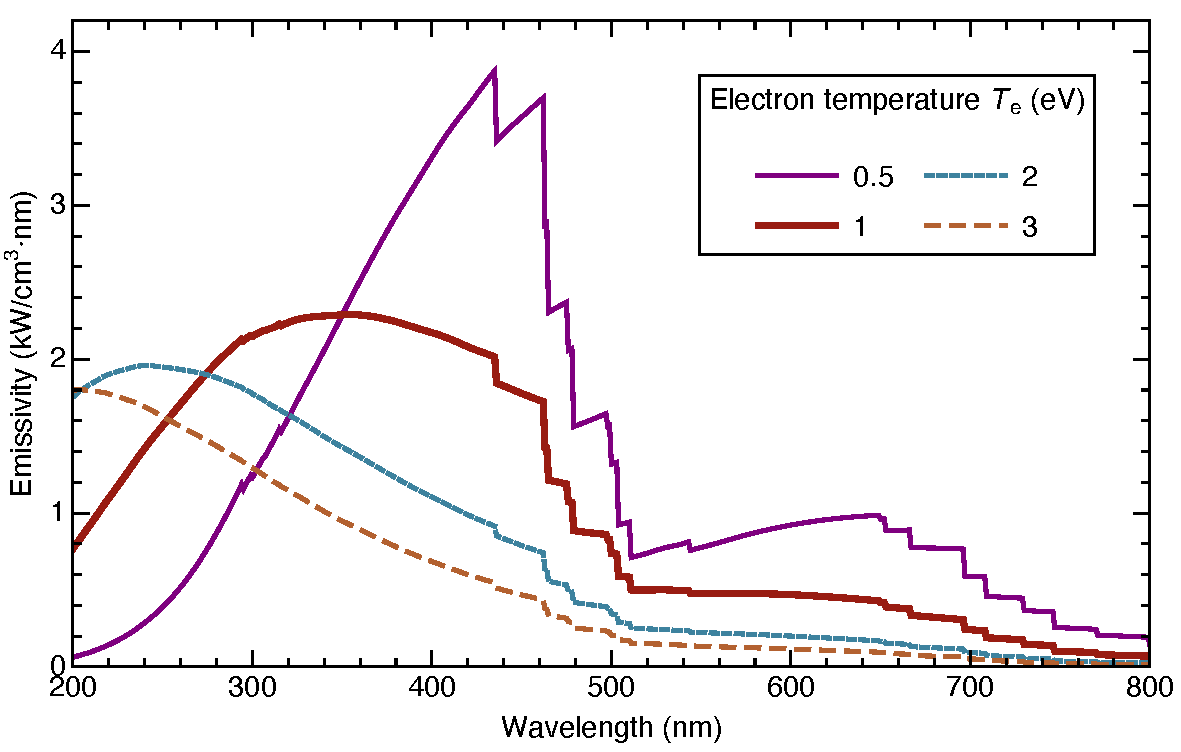
\includegraphics[width=100mm]{figures/ap6/recombination/continuum.pdf}
\caption{Recombination continuum of argon for different electron temperatures.}
\label{fig:recomContinuum}
\end{figure}

\begin{table}[]
\footnotesize
\centering
\begin{tabular}{lllll}
\hline \hline
Configuration    & Term        & J & g & Level (eV) \\ \hline \hline
3s$^\text{2}$3p$^\text{5}$(2P$^{\circ}_\text{3/2}$)4s & $^\text{2}${[}3/2{]}$^{\circ}$ & 2 & 5 & 11.54835442                                            \\
                 &             & 1 & 3 & 11.62359272                                            \\
3s$^\text{2}$3p$^\text{5}$(2P$^{\circ}_\text{1/2}$)4s & $^\text{2}${[}1/2{]}$^{\circ}$ & 0 & 1 & 11.72316039                                            \\
                 &             & 1 & 3 & 11.82807116                                            \\ \hline
3s$^\text{2}$3p$^\text{5}$(2P$^{\circ}_\text{3/2}$)4p & $^\text{2}${[}1/2{]}  & 1 & 3 & 12.90701530                                            \\
                 &             & 0 & 1 & 13.27303810                                            \\
3s$^\text{2}$3p$^\text{5}$(2P$^{\circ}_\text{3/2}$)4p & $^\text{2}${[}5/2{]}  & 3 & 7 & 13.07571571                                            \\
                 &             & 2 & 5 & 13.09487256                                            \\
3s$^\text{2}$3p$^\text{5}$(2P$^{\circ}_\text{3/2}$)4p & $^\text{2}${[}3/2{]}  & 1 & 3 & 13.15314387                                            \\
                 &             & 2 & 5 & 13.17177770                                            \\
3s$^\text{2}$3p$^\text{5}$(2P$^{\circ}_\text{1/2}$)4p & $^\text{2}${[}3/2{]}  & 1 & 3 & 13.28263902                                            \\
                 &             & 2 & 5 & 13.30222747                                            \\
3s$^\text{2}$3p$^\text{5}$(2P$^{\circ}_\text{1/2}$)4p & $^\text{2}${[}1/2{]}  & 1 & 3 & 13.32785705                                            \\
                 &             & 0 & 1 & 13.47988682                                            \\ \hline
3s$^\text{2}$3p$^\text{5}$(2P$^{\circ}_\text{3/2}$)3d & $^\text{2}${[}1/2{]}$^{\circ}$ & 0 & 1 & 13.8450385                                             \\
                 &             & 1 & 3 & 13.8636686                                             \\
3s$^\text{2}$3p$^\text{5}$(2P$^{\circ}_\text{3/2}$)3d & $^\text{2}${[}3/2{]}$^{\circ}$ & 2 & 5 & 13.9034546                                             \\
                 &             & 1 & 3 & 14.1525151                                             \\
3s$^\text{2}$3p$^\text{5}$(2P$^{\circ}_\text{3/2}$)3d & $^\text{2}${[}7/2{]}$^{\circ}$ & 4 & 9 & 13.9792373                                             \\
                 &             & 3 & 7 & 14.0127381                                             \\
3s$^\text{2}$3p$^\text{5}$(2P$^{\circ}_\text{3/2}$)3d & $^\text{2}${[}5/2{]}$^{\circ}$ & 2 & 5 & 14.0630272                                             \\
                 &             & 3 & 7 & 14.0990559                                             \\
3s$^\text{2}$3p$^\text{5}$(2P$^{\circ}_\text{1/2}$)3d & $^\text{2}${[}5/2{]}$^{\circ}$ & 2 & 5 & 14.2136715                                             \\
                 &             & 3 & 7 & 14.2361061                                             \\
3s$^\text{2}$3p$^\text{5}$(2P$^{\circ}_\text{1/2}$)3d & $^\text{2}${[}3/2{]}$^{\circ}$ & 2 & 5 & 14.2340226                                             \\
                 &             & 1 & 3 & 14.3036684                                             \\
\hline \hline
\end{tabular}
\caption{The three lowest excited states of argon atom \cite{kramida2020nist}.}
\label{table:argonStates}
\end{table}


